\documentclass[border=1pt]{standalone}
\usepackage{mathptmx}  % Times text and math
\usepackage{circuitikz}
\usetikzlibrary{arrows.meta}
\ctikzset{bipoles/length=0.75cm, transistors/scale=0.9,
  inductors/coils=4, current/distance=.5, bipoles/diode/height=.32,
  bipoles/diode/width=.26}
\begin{document}
\fontsize{8}{9.6}\selectfont
% mpc_fcs: control diagram, 1 layout unit = 1 cm (ieee-double)
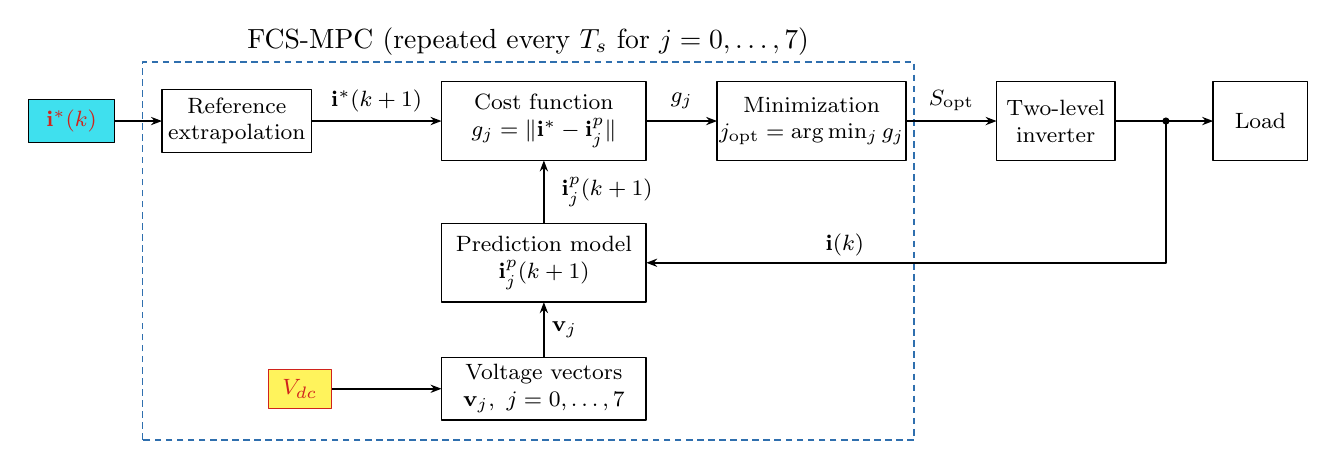
\begin{tikzpicture}[x=1cm, y=1cm, line width=0.55pt, line join=round]
% ---- regions (background) ----
\draw[draw={rgb,255:red,47;green,111;blue,174}, line width=0.44pt, dash pattern=on 2.4pt off 1.6pt] (1.6,-4.05) rectangle (11.4,0.75);
\node[inner sep=0pt] at (6.5,1.01) {FCS-MPC (repeated every $T_{s}$ for $j=0,\ldots,7$)};
% ---- links ----
\draw[-{Stealth[length=0.14cm]}] (1.25,0) -- (1.85,0);
\draw[-{Stealth[length=0.14cm]}] (3.75,0) -- (5.4,0);
\draw[-{Stealth[length=0.14cm]}] (8,0) -- (8.9,0);
\draw[-{Stealth[length=0.14cm]}] (11.3,0) -- (12.45,0);
\draw[-{Stealth[length=0.14cm]}] (13.95,0) -- (15.2,0);
\draw[-{Stealth[length=0.14cm]}] (14.6,0) -- (14.6,-1.8) -- (8,-1.8);
\draw[-{Stealth[length=0.14cm]}] (6.7,-1.3) -- (6.7,-0.5);
\draw[-{Stealth[length=0.14cm]}] (6.7,-3) -- (6.7,-2.3);
\draw[-{Stealth[length=0.14cm]}] (4,-3.4) -- (5.4,-3.4);
% ---- branch dots ----
\fill (14.6,0) circle (1.3pt);
% ---- iref (tag) ----
\filldraw[fill={rgb,255:red,63;green,224;blue,238}, draw={rgb,255:red,0;green,0;blue,0}, line width=0.33pt] (0.15,-0.275) rectangle (1.25,0.275);
% ---- extrap (block) ----
\draw[fill=white] (1.85,-0.4) rectangle (3.75,0.4);
% ---- cost (block) ----
\draw[fill=white] (5.4,-0.5) rectangle (8,0.5);
% ---- minim (block) ----
\draw[fill=white] (8.9,-0.5) rectangle (11.3,0.5);
% ---- inv (block) ----
\draw[fill=white] (12.45,-0.5) rectangle (13.95,0.5);
% ---- load (block) ----
\draw[fill=white] (15.2,-0.5) rectangle (16.4,0.5);
% ---- pred (block) ----
\draw[fill=white] (5.4,-2.3) rectangle (8,-1.3);
% ---- vv (block) ----
\draw[fill=white] (5.4,-3.8) rectangle (8,-3);
% ---- vdc (tag) ----
\filldraw[fill={rgb,255:red,255;green,243;blue,92}, draw={rgb,255:red,208;green,35;blue,28}, line width=0.33pt] (3.2,-3.65) rectangle (4,-3.15);
% ---- text ----
\node[inner sep=0pt, align=center, font=\fontsize{8}{9.6}\selectfont, text={rgb,255:red,208;green,35;blue,28}] at (0.7,0) {$\mathbf{i}^{*}(k)$};
\node[inner sep=0pt, align=center, font=\fontsize{8}{9.6}\selectfont] at (2.8,0) {Reference\\extrapolation};
\node[inner sep=0pt, align=center, font=\fontsize{8}{9.6}\selectfont] at (6.7,0) {Cost function\\$g_{j}=\|\mathbf{i}^{*}-\mathbf{i}^{p}_{j}\|$};
\node[inner sep=0pt, align=center, font=\fontsize{8}{9.6}\selectfont] at (10.1,0) {Minimization\\$j_{\mathrm{opt}}=\arg\min_{j} g_{j}$};
\node[inner sep=0pt, align=center, font=\fontsize{8}{9.6}\selectfont] at (13.2,0) {Two-level\\inverter};
\node[inner sep=0pt, align=center, font=\fontsize{8}{9.6}\selectfont] at (15.8,0) {Load};
\node[inner sep=0pt, align=center, font=\fontsize{8}{9.6}\selectfont] at (6.7,-1.8) {Prediction model\\$\mathbf{i}^{p}_{j}(k+1)$};
\node[inner sep=0pt, align=center, font=\fontsize{8}{9.6}\selectfont] at (6.7,-3.4) {Voltage vectors\\$\mathbf{v}_{j},\ j=0,\ldots,7$};
\node[inner sep=0pt, align=center, font=\fontsize{8}{9.6}\selectfont, text={rgb,255:red,208;green,35;blue,28}] at (3.6,-3.4) {$V_{dc}$};
\node[inner sep=0pt, align=center, font=\fontsize{8}{9.6}\selectfont] at (4.575,0.26) {$\mathbf{i}^{*}(k+1)$};
\node[inner sep=0pt, align=center, font=\fontsize{8}{9.6}\selectfont] at (8.45,0.26) {$g_{j}$};
\node[inner sep=0pt, align=center, font=\fontsize{8}{9.6}\selectfont] at (11.875,0.26) {$S_{\mathrm{opt}}$};
\node[inner sep=0pt, align=center, font=\fontsize{8}{9.6}\selectfont] at (10.52,-1.57) {$\mathbf{i}(k)$};
\node[inner sep=0pt, align=center, font=\fontsize{8}{9.6}\selectfont] at (7.5,-0.9) {$\mathbf{i}^{p}_{j}(k+1)$};
\node[inner sep=0pt, align=center, font=\fontsize{8}{9.6}\selectfont] at (6.96,-2.65) {$\mathbf{v}_{j}$};
\end{tikzpicture}
\end{document}
